\documentclass[tikz, border=10pt]{standalone}
\usepackage{pgfplots}
\usepackage{amsmath}
\usetikzlibrary{backgrounds}
\pgfplotsset{compat=1.18}

\begin{document}
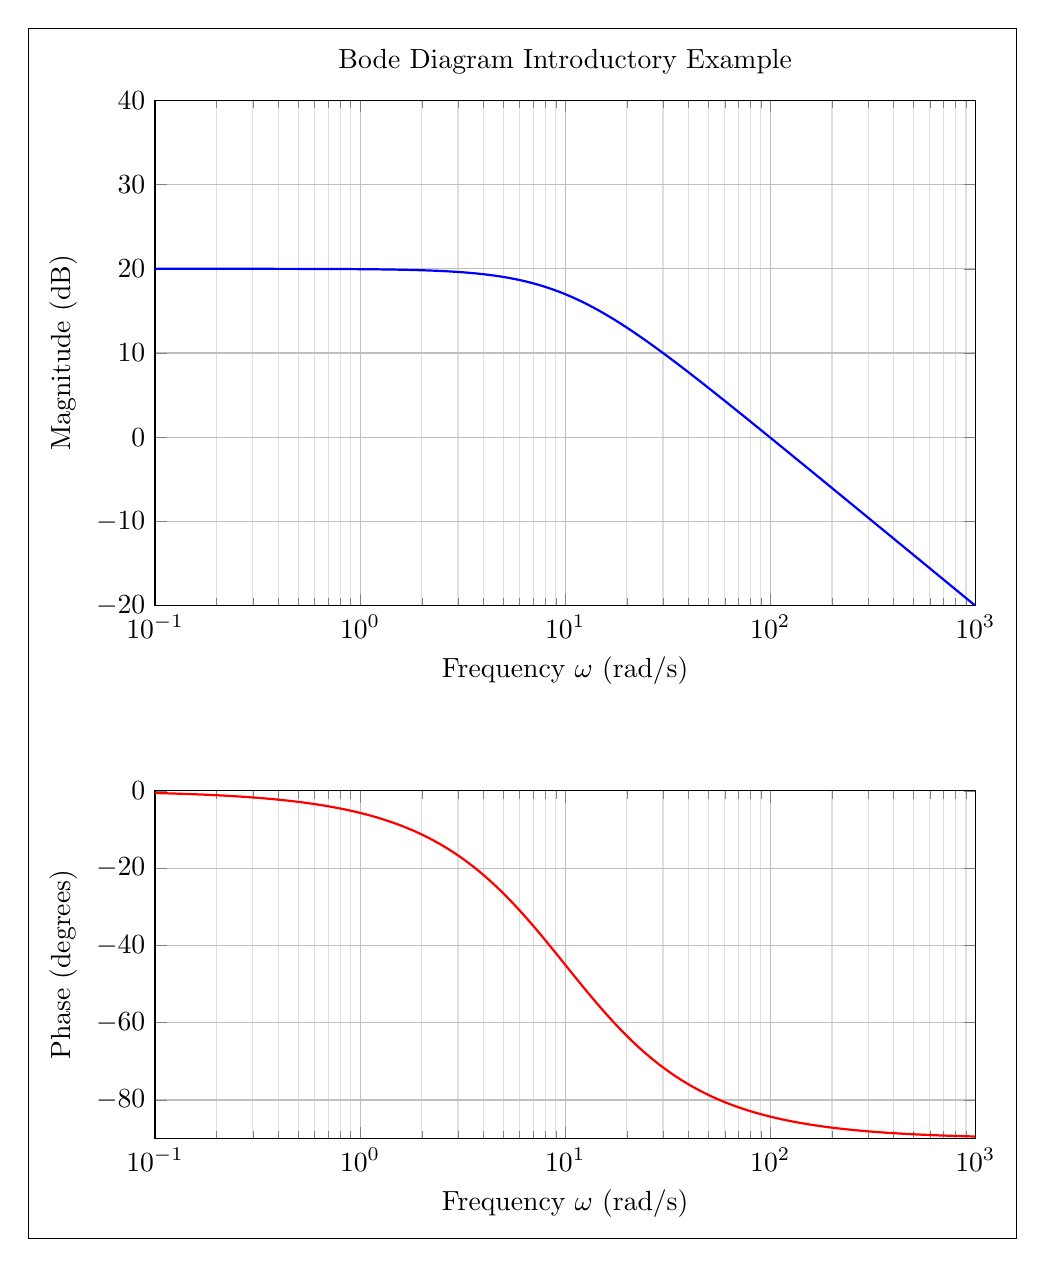
\begin{tikzpicture}[show background rectangle]
    \begin{axis}[
        width=12cm, height=8cm,
        at={(0,0)},
        name=magplot,
        title={Bode Diagram Introductory Example},
        xlabel={Frequency $\omega$ (rad/s)},
        ylabel={Magnitude (dB)},
        xmode=log,
        grid=both,
        xmin=0.1, xmax=1000,
        ymin=-20, ymax=40,
        minor grid style={gray!25},
        major grid style={gray!50},
    ]

    % Example plot: a simple low pass step or something representative
    % H(s) = 100 / (s + 10) = 10 / (1 + s/10)
    % Peak at low freq is 20 log 10 = 20 dB.
    \addplot[blue, thick, domain=0.1:1000, samples=200] { 20*log10( 10 / sqrt(1 + (x/10)^2) ) };
    
    \end{axis}
    
    \begin{axis}[
        width=12cm, height=6cm,
        at={(magplot.below south)},
        anchor=above north,
        yshift=-1cm,
        xlabel={Frequency $\omega$ (rad/s)},
        ylabel={Phase (degrees)},
        xmode=log,
        grid=both,
        xmin=0.1, xmax=1000,
        ymin=-90, ymax=0,
        minor grid style={gray!25},
        major grid style={gray!50},
    ]

    % Phase: -atan(x/10)
    \addplot[red, thick, domain=0.1:1000, samples=200] { -atan(x/10) };

    \end{axis}
\end{tikzpicture}
\end{document}
